% Connector --- What the software can do today (third-party briefing)
% Compile: make -C platform/docs/gtm -f Makefile.capability-report
% Honesty: docs/CONNECTOR_TRUTH_STORY.md · platform/products/catalog.json
% Must not say: court-green, SOC2 certified, LLM-as-CPU, finished multi-master mesh

\documentclass[10pt]{article}
\usepackage[margin=0.62in]{geometry}
\usepackage[T1]{fontenc}
\usepackage[utf8]{inputenc}
\usepackage{lmodern}
\usepackage{microtype}
\usepackage{enumitem}
\usepackage{booktabs}
\usepackage{array}
\usepackage{tabularx}
\usepackage{xcolor}
\usepackage{tikz}
\usepackage{colortbl}
\usepackage[hidelinks]{hyperref}
\usepackage{titlesec}

\usetikzlibrary{arrows.meta,positioning,fit}

\hypersetup{
  pdftitle={Connector --- What the software can do today},
  pdfauthor={Connector},
  pdfsubject={Third-party briefing: technical depth, operational use, economic diligence}
}

\definecolor{textmuted}{HTML}{475569}
\definecolor{navy}{HTML}{0F172A}
\definecolor{rule}{HTML}{CBD5E1}
\definecolor{ink}{HTML}{1E293B}
\definecolor{boxfill}{HTML}{F8FAFC}
\definecolor{kernel}{HTML}{E2E8F0}
\definecolor{ships}{HTML}{166534}
\definecolor{partial}{HTML}{92400E}
\definecolor{noclaim}{HTML}{475569}
\definecolor{warnbg}{HTML}{FEF3C7}
\definecolor{infobg}{HTML}{EFF6FF}

\setlength{\parindent}{0pt}
\setlength{\parskip}{0.42em}
\setlist[itemize]{nosep,leftmargin=1.15em,itemsep=0.10em,topsep=0.16em,parsep=0pt}
\setlist[enumerate]{nosep,leftmargin=1.2em,itemsep=0.10em,topsep=0.16em,parsep=0pt}
\titleformat{\section}{\normalfont\bfseries\fontsize{12}{14}\selectfont\color{navy}}{\thesection.}{0.5em}{}
\titlespacing*{\section}{0pt}{1.05em}{0.32em}
\titleformat{\subsection}{\normalfont\bfseries\fontsize{10.5}{13}\selectfont\color{navy}}{\thesubsection.}{0.45em}{}
\titlespacing*{\subsection}{0pt}{0.72em}{0.22em}

\newcommand{\muted}[1]{\textcolor{textmuted}{#1}}
\newcommand{\ships}{\textcolor{ships}{\textbf{Ships today}}}
\newcommand{\partialm}{\textcolor{partial}{\textbf{Partial}}}
\newcommand{\noclaim}{\textcolor{noclaim}{\textbf{Not a claim}}}

\begin{document}
\pagestyle{empty}
\thispagestyle{empty}

{\fontsize{18}{21}\selectfont\bfseries\color{navy} What Connector can do today}\\[0.18em]
{\fontsize{11.5}{14}\selectfont\bfseries The operating layer for intelligence that already acts}\\[0.28em]
{\small\muted{Third-party briefing --- August 2026. Technical depth, operational usefulness, and economic diligence. Honest product bar: single-node OS.}}

\vspace{0.22em}
\noindent{\color{rule}\rule{\linewidth}{0.7pt}}

\vspace{0.35em}
\noindent\colorbox{infobg}{\parbox{\dimexpr\linewidth-2\fboxsep\relax}{%
\textbf{The sentence a stranger can keep.} Connector is a self-hosted AI operating system node. Teams install one machine (or one VM). Agents, models, tools, workflows, and plugins then run under shared identity, admission, isolation, memory, audit, and usage truth. DevGuard, TraceTramp, and WitnessCtl are institutions on that node --- not a second platform, and not a pile of dashboards taped together.}}

\vspace{0.45em}
\noindent
\begin{tabularx}{\linewidth}{@{}>{\centering\arraybackslash}X >{\centering\arraybackslash}X >{\centering\arraybackslash}X >{\centering\arraybackslash}X@{}}
{\fontsize{13}{15}\selectfont\bfseries 1 node} &
{\fontsize{13}{15}\selectfont\bfseries L3 / L4} &
{\fontsize{13}{15}\selectfont\bfseries 3 apps} &
{\fontsize{13}{15}\selectfont\bfseries Not L5} \\
{\footnotesize\muted{Installable SKU}} &
{\footnotesize\muted{Honest maturity bar}} &
{\footnotesize\muted{First-party governance}} &
{\footnotesize\muted{Mesh / court-grade not claimed}}
\end{tabularx}

\section{Connector, crisply}

\textbf{What it is.} Connector is a self-hosted operating substrate for intelligence that already acts. It is the layer that sits beneath agents, models, tools, workflows, and plugins so those things can run under shared identity, admission, isolation, memory, audit, and usage truth.

\textbf{What it is made for doing.}
\begin{itemize}
  \item Turn an agent from a prompt-driven application into a governed process with a real identity, limits, and lifecycle.
  \item Put a policy boundary in front of effects such as tool calls, writes, network actions, approvals, and spending.
  \item Give operators one origin for model traffic, workflow execution, plugin installation, traces, receipts, and runtime inspection.
  \item Let developers build installable intelligence software --- workflows, contracts, rules, and agent apps --- that can be verified and run on a real node.
  \item Keep the control layer sovereign: self-hosted, operator-owned, and usable without requiring a hyperscale service maze.
\end{itemize}

\textbf{What outcome it creates today.} Teams can run one governed node, point existing OpenAI-compatible clients at it, register agents, enable workflows, install signed \texttt{.cpkg} packages, trace execution, seal receipts, and govern developer tools from the same substrate.

\textbf{What future outcome it is aiming at.} Over time, the same operating model should make intelligence infrastructure composable across more nodes, more geographies, more institutions, and more regulated actions --- without losing identity, auditability, resource truth, or operator control.

\textbf{Why the deeper idea matters even beyond Connector.} The lasting point is not this product name. The lasting point is that agentic systems need an operating architecture, not only a framework. As software moved from raw programs to operating systems, intelligence software will also need standard primitives: identity, memory boundaries, admission, receipts, resource accounting, isolation, and installable packages. Even if a future industry standard is built by others, this architectural idea --- that intelligence must run on a governed substrate --- is likely to become fundamental.

\section{The problem it exists to solve}

Most teams now run agents the way early computers ran programs: the model talks, a framework calls tools, and the rest is hoped for. Identity is a prompt. Memory is a chat window or a RAG index. Policy is a Python if-statement. Audit is a log file. Cost is a guess in a sidebar. Isolation is ``maybe Docker.''

That is tolerable while agents only draft email. It becomes expensive the moment they touch production systems, customer data, codebases, or spend. Then each missing OS primitive shows up as a leak, a runaway bill, a fake-green compliance dashboard, or an incident nobody can reconstruct.

Connector exists so intelligence can be treated as a \textbf{process on a kernel}, not a chatbot with plugins. The agent does not own the operating system. The node does.

\section{What it is, in ordinary language}

Think of Windows or Linux, but for agents. An operator installs \texttt{connector-platform} and \texttt{connectorctl}, opens the embedded dashboard, and has one origin for everything agentic. Existing OpenAI-compatible clients can point their \texttt{base\_url} at the node. Python developers can author apps with Gloo, package them as \texttt{.cpkg} installers, and burn workflows into the same registry as first-party apps.

\vspace{0.25em}
\begin{center}
\resizebox{\linewidth}{!}{%
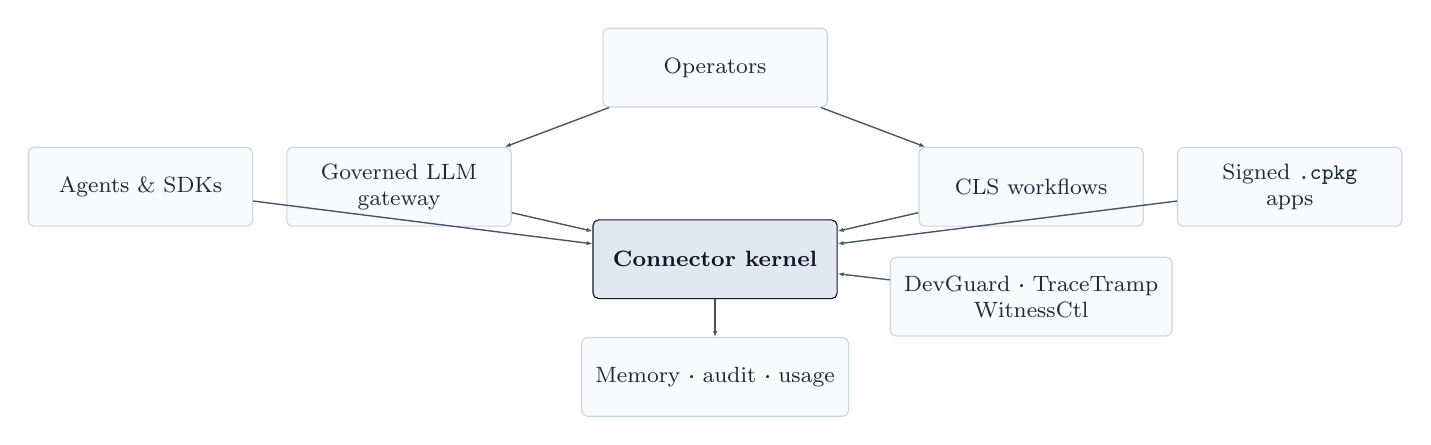
\begin{tikzpicture}[
  font=\footnotesize,
  node/.style={draw=rule, fill=boxfill, rounded corners=2pt, inner sep=5pt, align=center, text=ink, minimum height=1.0cm, minimum width=2.85cm},
  knode/.style={draw=navy, fill=kernel, rounded corners=2pt, inner sep=5pt, align=center, text=navy, font=\footnotesize\bfseries, minimum height=1.0cm, minimum width=3.1cm},
  arr/.style={-{Latex[length=2.1pt]}, color=textmuted, line width=0.5pt}
]
\node[node] (ops) {Operators};
\node[node, below left=0.50cm and 1.15cm of ops] (gw) {Governed LLM\\gateway};
\node[node, below right=0.50cm and 1.15cm of ops] (wf) {CLS workflows};
\node[node, left=0.42cm of gw] (ag) {Agents \& SDKs};
\node[node, right=0.42cm of wf] (pl) {Signed \texttt{.cpkg}\\apps};
\node[node, below=0.38cm of wf] (ins) {DevGuard · TraceTramp\\WitnessCtl};
\node[knode, below=1.42cm of ops] (k) {Connector kernel};
\node[node, below=0.48cm of k] (mem) {Memory · audit · usage};

\draw[arr] (ops) -- (gw);
\draw[arr] (ops) -- (wf);
\draw[arr] (ag) -- (k);
\draw[arr] (gw) -- (k);
\draw[arr] (wf) -- (k);
\draw[arr] (ins) -- (k);
\draw[arr] (pl) -- (k);
\draw[arr] (k) -- (mem);
\end{tikzpicture}%
}
\end{center}
{\footnotesize\muted{Source: Connector product architecture as shipped in-tree, August 2026. The kernel is the system of record. Apps sit on top.}}

\vspace{0.35em}
\renewcommand{\arraystretch}{1.18}
{\small
\begin{tabularx}{\linewidth}{@{}>{\bfseries\arraybackslash}p{0.18\linewidth} X >{\raggedright\arraybackslash}p{0.16\linewidth}@{}}
\toprule
Layer & What ships & Status \\
\midrule
Node & One tarball. One process group. Embedded operator dashboard. CLI for start, stop, backup, hub, and diagnosis. Runs in a VPC, localhost, or air-gapped posture. Kubernetes is optional packaging, not the product. & \ships \\
Kernel & Admission in front of effects. Agent registry with PIDs. Content-addressed memory. Governed LLM gateway. Workflow lifecycle. Usage books that refuse to invent \$0. Isolation cages for plugins. & \ships \\
Institutions & DevGuard locks down tool and host actions. TraceTramp records execution. WitnessCtl seals receipts. They share the same identity, policy, and evidence primitives instead of each inventing a private universe. & Apps on the OS \\
\bottomrule
\end{tabularx}}

\section{What people can do with it today}

Capabilities below are written for a buyer or operator who has never seen the codebase. \ships\ means it is in running software. \partialm\ means the surface exists but should not be sold as finished. \noclaim\ is something a diligent reader should refuse to buy against.

\renewcommand{\arraystretch}{1.16}
{\small
\begin{tabularx}{\linewidth}{@{}>{\bfseries\arraybackslash}p{0.24\linewidth} X >{\raggedright\arraybackslash}p{0.16\linewidth}@{}}
\toprule
Job & What that means in practice & Maturity \\
\midrule
Install and operate one node & Unpack, start, open the dashboard, inspect health. No service maze required to get a governed origin. & \ships \\
Put existing agents behind a gate & Point OpenAI-compatible clients at the node gateway. Every call is attributed to a Connector principal, not an anonymous SDK. & \ships \\
Choose any model backend & Link OpenAI, Anthropic, Gemini, Ollama, LM Studio, vLLM, or a custom OpenAI-compatible endpoint. The model is a provider. Identity stays in Connector. & \ships \\
Charter and register agents & Give an agent a name, purpose, namespace, model, tools, and limits before it can act. It becomes a process, not a prompt. & \ships \\
Author governed workflows & Write CLS (Connector Contract Language), compile, dry-run, enable, pause, archive. Workflows are programs on the node, with version history. & \ships \\
Install signed software packages & A \texttt{.cpkg} is verified (manifest, optional Ed25519, dependency check), installed into a cage, and --- for Gloo apps --- burned into the workflow registry with system-default importance. & \ships \\
Trace live execution & TraceTramp records decisions, tool calls, and LLM exchanges with timestamps. Operators can search by agent, not grep twelve log files. & \ships \\
Seal evidence & WitnessCtl issues signed receipts. Useful for internal audit and reconstruction. Not marketed as court-grade custody. & \partialm \\
Guard developer tools & DevGuard mediates coding-agent actions (secrets, shell, egress). Same policy lineage as production, not a separate browser-extension story. & \partialm \\
Meter spend without lying & Usage events and books exist. Unavailable data is not rendered as \$0. Exact provider invoices require a rate card. & \partialm \\
Human-in-the-loop & Risky steps can be held for approval. Inbox and resume paths exist; a single polished operator inbox is still being unified. & \partialm \\
Global multi-node mesh & Cell-boot and membership foundations exist in code. Honesty APIs still report \texttt{single\_node}. Do not buy this as a finished HA product. & \noclaim \\
\bottomrule
\end{tabularx}}

\vspace{0.12em}
{\footnotesize\muted{Source: in-tree product surfaces and honesty APIs, August 2026. Maturity labels follow the Connector truth story, not marketing copy.}}

\section{Operational usefulness}

The useful question is not ``does it have AI.'' It is whether a platform team can run intelligence like they run any other production substrate. Connector's answer is a single origin with four operator jobs.

\renewcommand{\arraystretch}{1.14}
{\small
\begin{tabularx}{\linewidth}{@{}>{\bfseries\arraybackslash}p{0.22\linewidth} X >{\raggedright\arraybackslash}p{0.32\linewidth}@{}}
\toprule
Persona & What they do & Success looks like \\
\midrule
ML / platform engineer & Register providers, mint a scoped key, point existing agents at the gateway. Get traces and cost attribution without forking every repo to add a tracing SDK. & One gateway URL, fallback routing, and TraceTramp search instead of a private Prometheus for prompts. \\
Security / compliance & High-risk tool paths can require a receipt or a human step, expressed as a workflow the legal team can read --- not a Python script only one engineer understands. & Policy version + principal + evidence in one place, not twelve application logs. \\
Automation engineer & CLS workflows have lifecycle: draft, compile, stage, enable, pause, archive. Dry-run shows what would have fired. Gloo packages install like apps and register as first-class workflows after Connector checks pass. & Enable / rollback, not a spreadsheet of shell history. \\
Staff developer & DevGuard binds coding agents to the same node. Local tool calls can be allowed, blocked with a reason, or routed through the gateway. Policy IDs can match staging. & One policy lineage from IDE to cluster, not a different story in every tool. \\
\bottomrule
\end{tabularx}}

\section{Technical depth, without the jargon wall}

Under the dashboard is a real kernel shape, not a web app with a ``governance'' tab. The important primitives are ordinary OS ideas, applied to intelligence.

\renewcommand{\arraystretch}{1.14}
{\small
\begin{tabularx}{\linewidth}{@{}>{\bfseries\arraybackslash}p{0.20\linewidth} p{0.34\linewidth} X@{}}
\toprule
OS idea & Connector equivalent & Why it is not optional \\
\midrule
Process identity & Agent PID, intelligence charter, scoped API keys & Without it, every model invents a name and every tool call is anonymous. \\
Syscall boundary & Admission + CNP dispatch tokens for workflows & Effects (write, spend, share, tool) must be allow / deny / hold, with a reason. \\
Memory protection & Namespaced MemPackets, moments, Object Fabric CAS & Agent A must not read Agent B. Memory must survive a crash and remain addressable. \\
Filesystem / packages & Signed \texttt{.cpkg}, \texttt{plugin.toml}, cage extract, Hub & Extensions are untrusted code. They install like apps, not like \texttt{curl | bash}. \\
Audit log & Keyed HMAC chain, TraceTramp traces, WitnessCtl receipts & Logs that the producer can silently edit are not evidence. \\
Resource accounting & Usage events, books, budget posture & A missing meter rendered as \$0 is a liability, not a feature. \\
Isolation & Plugin cages, microVM default in production posture & An agent with tools is a network-capable program. Containment has to be declared. \\
\bottomrule
\end{tabularx}}

\vspace{0.28em}
\noindent\colorbox{boxfill}{\parbox{\dimexpr\linewidth-2\fboxsep\relax}{%
\textbf{What Gloo is in this picture.} Gloo is the Python developer environment on top of the node: scaffold an app, write CLS workflows, contracts, policies, identity and address rules, build a verified \texttt{.cpkg} with a hash-chained receipt ledger, then install it onto a real Connector address (localhost, Kubernetes, or cloud). After Connector checks pass, workflows burn into the registry with the same operational class as DevGuard, TraceTramp, and WitnessCtl. Gloo is not a second kernel. It is how developers write programs for this OS.}}

\section{Economic diligence}

Connector is bought as infrastructure, not as a model. Diligence should compare it to the cost of assembling the missing OS from parts --- and to the cost of pretending those parts already exist.

\subsection{What a buyer is actually paying for}

\textbf{One SKU:} a self-hosted node license (\texttt{connector-platform} + \texttt{connectorctl}). Not a GPU farm --- models stay customer-chosen. Not a chatbot --- the kernel sits under existing agents.

Customers keep LangGraph, Crew, vLLM, Ollama, OpenAI, MCP. Connector sits \textbf{beneath} them: charter, admit, remember, stop, prove. That is the economic claim. It is not ``we replace your model vendor.''

\subsection{Cost of the substitute assembly}

\renewcommand{\arraystretch}{1.14}
{\small
\begin{tabularx}{\linewidth}{@{}>{\bfseries\arraybackslash}p{0.26\linewidth} X >{\raggedright\arraybackslash}p{0.30\linewidth}@{}}
\toprule
Without Connector & Hidden cost & With Connector \\
\midrule
Framework + prompt policy & Policy lives in app code; every team forks it; no shared deny reason. & Admission and CLS workflows are node-level programs. \\
Observability sidecar per service & Prompt logs in five formats; no common principal; spend is a spreadsheet. & Gateway attribution + TraceTramp on the same origin. \\
SIEM + log export as ``audit'' & Producer-controlled logs. Auditors cannot recompute. Incidents do not reconstruct. & Receipts and keyed audit chains. Honesty about what is not yet court-grade. \\
Cloud secret + \texttt{.env} sprawl & Keys in process environments, laptops, and plugin cages. & Vault on the node; bootstrap migration off env vars. \\
FinOps after the invoice & Runaway agent loops discovered at month-end. Fake \$0 when meters fail. & Usage-first books; unavailable $\neq$ \$0; cost-cap posture on the gateway. \\
IDE guard as a separate SKU & Laptop policy diverges from production. Developers route around it. & DevGuard bound to the same node and policy IDs. \\
\bottomrule
\end{tabularx}}

\vspace{0.08em}
{\footnotesize\muted{This table is qualitative. It does not invent dollar savings. The economic case is avoided duplication plus avoided incident class --- not a fabricated ROI percentage.}}

\subsection{What a careful buyer should refuse}

\vspace{0.12em}
\noindent\colorbox{warnbg}{\parbox{\dimexpr\linewidth-2\fboxsep\relax}{%
\textbf{Claims Connector itself does not authorize.} Do not underwrite SOC~2 certified, court-grade chain of custody, automatic multi-region failover, global multi-master mesh, or ``the LLM is the CPU.'' Those are either future targets or other companies' slogans. Honesty APIs still report a single node. Witness receipts are real software; they are not a finished legal product. Usage panels are meters, not your cloud bill.}}

\subsection{Why the architecture is economically conservative}

The product is designed so a determined operator can run the whole system without a hyperscale estate. One node, local and VPC operation, modest-resource paths, explicit processes, and a plugin economy that independent developers can target. That is not romantic. It is a cost and sovereignty choice: intelligence infrastructure should not require renting a maze of vendor control planes to be allowed to act.

The counter-risk is also real. A kernel this wide can look complete while some journeys remain partial (unified inbox, live workflow worker versus recorded enablement, mesh, commercial trial conversion). Diligence should score Connector as a \textbf{strong single-node operating layer with institutions on top} --- then fund or wait for the gaps that match the buyer's actual risk, not a slide that says ``platform.''

\section{How a third party should remember it}

\renewcommand{\arraystretch}{1.16}
{\small
\begin{tabularx}{\linewidth}{@{}>{\bfseries\arraybackslash}p{0.12\linewidth} X@{}}
\toprule
It is & An installable operating substrate for agents that already act. Identity, admission, memory, workflows, signed packages, traces, receipts, and usage live on one node. Developers write programs for it. Operators run it like infrastructure. \\
\midrule
It is not & A better LangGraph, a GPU cloud, a chat product, or a finished planetary mesh. Those can sit on it, or come later. Buying Connector for those jobs is the wrong diligence conclusion. \\
\bottomrule
\end{tabularx}}

\vspace{0.55em}
{\fontsize{11}{14}\selectfont\bfseries\color{navy} If intelligence is going to write to the world, someone has to be the operating system. Connector is the attempt to make that layer real, inspectable, and owned by the operator who runs the node.}

\vspace{0.55em}
\noindent{\color{rule}\rule{\linewidth}{0.5pt}}\\[0.4em]
{\footnotesize\muted{Prepared from Connector's in-tree truth story, product catalog, and shipped kernel surfaces. August 2026. Claims above L4 / multi-node mesh remain unsigned. This page is a briefing, not a certificate.}}

\end{document}
